\chapter{Access Control Techniques}
\label{AccessControlTechniques}
\begin{itemize}
 \item \textbf{Mandatory Access Control:} controllo d'accesso generalizzato
 (determinato dal sistema). Specifica di chi può accedere a cosa;
 \item \textbf{Discretionary Access Control:} permette ad un individuo
 designato di decidere il livello di accesso degli utenti.
 Si trova spesso dove l'informazione deve essere classificata;
 \item \textbf{Role-Based Access Control:} il controllo di accesso è
 determinato dal ruolo che si ricopre all'interno dell'organizzazione.
 Questa è la soluzione migliore per i contesti
 organizzativi classici. Essendoci un numero fissato di ruoli, per
 l'amministratore di sistema la loro gestione diviene più semplice,
 perché non deve gestire ogni singolo impiegato.
 Questa realtà è ancora in forte sviluppo;
 \item Physical Access Control: è quell’area legata alla sicurezza
 fisica, ed è legata al CISO ultimamente\footnote{Ricordiamo al lettore
 come precedentemente questa responsabiltà era coperta dal CSO, che sta
 pian piano venendo soppiantato dal CISO.}. Si costituisce di lucchetti,
 chiavi, ecc.

\end{itemize}


\section{Role-Based Access Control}

Prima di mettersi a fare controlli sugli accessi bisogna prima comprendere per
bene quali ruoli sono presenti all'interno dell'azienda (analisi interna).

\begin{table}[H]
\centering
\resizebox{\textwidth}{!}{%
\begin{tabular}{|l|p{10cm}|}
\hline
\textbf{Nome del ruolo} & \textbf{Informazioni d'accesso e permessi (R=read,
W=write)} \\
\hline
Istruttore & Form dei voti RW; Esami sostenuti dallo studente R; Trasferimento
di crediti R \\
\hline
Consigliere & Esami sostenuti dallo studente R; Pagamento tasse R;
Trasferimento di crediti R \\
\hline
Registratore & Pagamento tasse RW; Trasferimento di crediti RW \\
\hline
\end{tabular}%
}
\caption{Un esempio di un \textit{Role-Based Access Control}}
\end{table}



\section{Military Security Policy}

Si applica una classificazione dell'informazione, che può essere:
\begin{itemize}
 \item Top secret;
 \item Secret;
 \item Confidential;
 \item Non-classified.
\end{itemize}

Per evitare l'\textit{overclassification} si utilizzano i domini: si cercano
di mettere delle persone con determinate competenze nel contesto giusto (es.
se un dominio è il nucleare e io non ho competenze a riguardo non posso
accedere a quel dominio).

Un soggetto può accedere ad un oggetto solo se domina (maggiore o uguale) la
classificazione dell'oggetto.

\section{Modello Bell-La Padula}

Si è dimostrato che adottando questo modello possiamo avere buone proprietà di
confinamento dell'informazione.\\
Utilizza il principio di confidenzialità: si può avere accesso in lettura a
tutto ciò che dominiamo. Per la scrittura invece vale il contrario: posso
accedere in scrittura a tutto ciò che mi domina ma non posso scrivere a ciò che
domino. Il tutto viene riassunto in \textit{no read up} e \textit{no write
down}.\\
\newline
\textbf{Principio di tranquillità:} le classi degli oggetti non possono
cambiare.\\
\newline
La declassificazione risolve il problema del galleggiamento verso l'alto. Avere
troppi documenti top-secret può causare problemi. Eseguire una
declassificazione è una procedura costosa, ed è quando il livello di segretezza
di un certo documento viene abbassato.

\section{System Access Control}

Il \textit{System Access Control} si occupa di:
\begin{itemize}
  \item stabilire le regole di accesso alle informazioni;
  \item creare e manutenere i profili degli utenti;
  \item dare gli ID agli utenti per l'autenticazione;
  \item informare gli utenti su come accedere e utilizzare il sistema in modo
  valido, prima e dopo il login;
  \item accertare la responsabilità registrando l'attività degli utenti;
  \item eseguire il log degli eventi;
  \item generare report per l'amministrazione di sistema dei tentativi falliti
  di accesso, che possono essere anche accidentali.
\end{itemize}

\section{Application-Level Access Control}

Gli obiettivi del \textit{application-level access control} sono:
\begin{itemize}
 \item creare/cambiare file o struttura del database;
 \item autorizzare azioni al livello di
  \begin{itemize}
   \item applicazione;
   \item file;
   \item transazione;
   \item campo;
  \end{itemize}
\item log di accessi alla rete e ai dati.
\end{itemize}

\section{Password}
\label{Password}

\subsection{Tutto quello che avreste voluto sapere ma non avete mai osato
chiedere sulle password}

Cos'è una password? Una sequenza arbitraria di caratteri segreta e difficile da
indovinare.

Ancora al tempo di Venezia era presente una sezione di cifratura
apposita. Oggi, l'NSA è l'istituzione che ha più matematici al mondo.

\subsubsection{Gestione delle password}

Le password servono a discriminare chi ha diritto o no ad accedere al servizio.
Le password nei sistemi vengono solitamente cifrate e salvate, in questa
maniera non è presente la password in chiaro. Per eseguire ciò di solito si
eseguono delle tecniche di \textit{hashing}.

\subsubsection{Difficoltà delle password}

Con una password da N caratteri, in cui ogni carattere può assumere M valori,
abbiamo $N^M$ possibili password.

\subsection{Come creare una buona password}

Le password scelte dagli utenti non sono solitamente forti, ma tendono ad
essere deboli e ripetitive. La bontà di una password dipende anche dalla sua
\textit{entropia}.
Le password solitamente sono simili a quelle di nomi di persone, date di
nascite o numeri di telefono.

\paragraph*{Base words}
Le \textit{base-words passwords} sono password significative dal punto di vista
mnemonico che risultano essere difficili da indovinare da un attaccante perché
per un estraneo risultano come se fossero una combinazione casuale di parole.
È un metodo molto valido per costruire una forte password.

\paragraph*{Facciamo i conti}

Il dizionario inglese ha 170 mila parole, vuol dire che se combiniamo 2 parole
abbiamo 29 miliardi di tentativi per indovinare per password. Il problema è che
le GPU moderne possono provare fino a 40 miliardi di password al giorno.
È possibile attaccare oggi come oggi sistemi molto difesi tramite attacchi di
forza bruta.
$2^{80}$ è il limite teorico oltre il quale un sistema è considerato
inattaccabile. Una password di 10 caratteri con 46 possibili caratteri ha circa
$2^{55}$ possibilità.

\paragraph*{Attacco del dizionario}
Le password sono solitamente deboli all'attacco del dizionario: ovvero sono
password che hanno al loro interno pattern di persone/cose (come ad esempio il
nome di una serie TV o simili). I dizionari al giorno d'oggi sono addirittura
comprabili, e presentano tutte le entry di un determinato campo semantico.
È meglio quindi evitare l'uso di password che abbiano pattern al loro interno.
È meglio la generazione di una password totalmente casuale.

\subsection{Autenticazione a due fattori}

Esistono differenti metodi per autenticarsi, e una buona autenticazione si
basa su diversi aspetti, detti fattori. Se si basa su un singolo fattore viene
detta \textit{single factor authentication} (es. una password), mentre si
parla di \textit{multifactor authentication} quando se ne utilizza più di uno.

I fattori sono:
\begin{itemize}
 \item \textbf{Qualcosa che siamo} (es. impronte biometriche);
 \item \textbf{Qualcosa che abbiamo} (es. una chiavetta);
 \item \textbf{Qualcosa che sappiamo} (es. una password).
\end{itemize}
L'autentificazione è detta \emph{forte} quando è ad almeno due fattori, e
solitamente si utilizza \emph{qualcosa che si ha} (es. un ID) e \emph{qualcosa
che si è} (es. impronte digitali). Questa funziona bene perché, in questo
modo, sono due i canali che devono essere compromessi da un attaccante per
ottenere l'accesso.

Un altro esempio è l'autenticazione bancaria che, al giorno d'oggi, richiede
solitamente il proprio codice bancario e un altro codice proveniente da una
chiavetta/sms/token hardware.

Una nuova tecnica è anche quella della autorizzazione tramite
geolocalizzazione. Sempre nell'ambito bancario, pagamenti eseguiti a breve
tempo da diverse parti del mondo non vengono autorizzati.

\subsection{Single Sign On}
Il Single Sign On (SSO) serve per poter accedere a una serie di servizi offerti dal
provider. Con il SSO è il segmento con cui ci si autentica per primi che
fornisce l'autorizzazione anche per le altre applicazioni.
La sicurezza che il SSO offre non è la stessa della segmentazione dei
servizi.

I \textbf{vantaggi} di questa tecnica:
\begin{itemize}
\item una buona password rimpiazza molte password;
\item ID consistente tra i sistemi;
\item riduce il lavoro degli admin nel setup e per le password dimenticate;
\item accesso rapido ai sistemi.
\end{itemize}



Gli \textbf{svantaggi}:
\begin{itemize}
\item Single Point of Failure (\textbf{SPOF});
\item Lo sviluppo del software è complicato per via di diversi sistemi
operativi;
\item Implementazione onerosa.
\end{itemize}

\subsection{Biometria}

È molto utile per eseguire autenticazioni, ma funziona ancora male in contesti
quali per esempio le riprese di sicurezza.

Chi sei e cosa fai, è suscettibile ad errori.

\begin{itemize}
\item \textbf{False Rejection Rate} (FRR): anche detto
\textbf{falso negativo}, un reject che non dovrebbe esserci stato;
\item \textbf{False Acceptance Rate} (FAR): anche detto
\textbf{falso positivo}, un accept quando non avrebbe dovuto esserci;
\item \textbf{Failure to Enroll Rate:} numero di utenti che non sono
riusciti a registrarsi correttamente.
\item \textbf{Equal Error Rate} (ERR): impostazione usata
in biometria, per aggiustare la sentività del sistema per avere
FRR e FAR equivalenti.
\end{itemize}
La relazione tra FRR, FAR e ERR vengono riassunte nella Figura
\ref{fig:equalErrorRate}.

\begin{figure}[H]
 \centering
 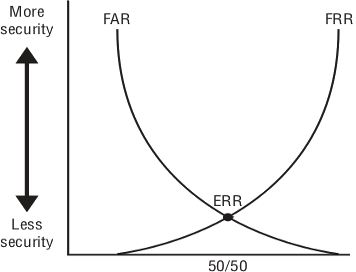
\includegraphics[scale=0.8]{equal_error_rate}
 \caption{Relazione tra Equal Error Rate, False Rejection Rate e
 False Acceptance Rate.}
 \label{fig:equalErrorRate}
\end{figure}


\subsubsection{Metodi migliori per l'autenticazione}

\begin{figure}[H]
 \centering
 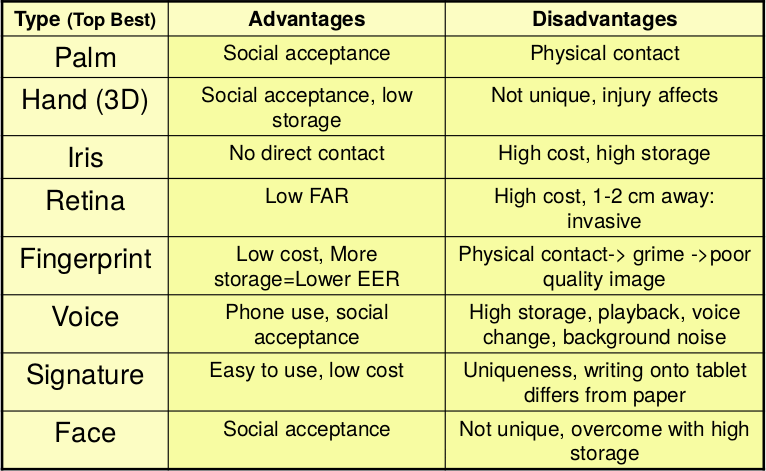
\includegraphics[scale=0.425]{best_biometrics_table}
 \caption{Confronto tra le varie biometrie rispetto a tempo di risposta e EER
(\emph{Equal Error Rate}) più basso. }
\end{figure}


\subsubsection{Biometric Info Management \& Security (BIMS) Policy}

\begin{itemize}
 \item Procedure di identificazione e autenticazione:
 \item Backup delle autenticazioni (es. non chiedere l'autenticazione ogni
 volta);
 \item Trasmissione/conservazione sicura dei dati biometrici;
 \item Sicurezza fisica dell'hardware;
 \item Test di valutazione.
\end{itemize}

I dispositivi per la cattura del viso per esempio stanno in aree aperte, e se
un attaccante è in grado di manomettere il dispositivo ha la possibilità di
inserire un dispositivo di acquisizione personale, per poter registrare i dati
e ottenerli in maniera non autorizzata. In questa maniera l'attaccante è in
grado di eseguire un furto d'identità. Questi strumenti dovrebbero essere posti
in aree controllate, cosa che spesso non succede. È importante che l'integrità
di questi strumenti venga mantenuta.

\subsection{Verifiche di un IS Auditor}
\begin{itemize}
 \item Verificare che ci siano delle procedure e che siano implementate;
 \item Verificare che i processi seguano il pattern del \textit{need to know};
 \item Security awareness e training implementati;
 \item Il data owner e il data custodian devono sapere di essere responsabili
 della salvaguardia dei dati;
 \item Il security administrator deve fornire la sicurezza fisica e logica per
 il programma IS, i dati e l'equipaggiamento;
 \item Le autorizzazioni devono essere documentate e consistenti con la realtà.
\end{itemize}


\section{Esercizi}

Gli esercizi sono disponibili nella Sezione \ref{EsPass}.
